\documentclass[a4paper,11pt]{report}

\def\Author{Andreas Bock, bock@andreasbock.dk\\
Johan Astborg, joastbg@gmail.com\\\\
Supervisors:\\
Jost Berthold, jb.diku@gmail.com\\
Sinan Gabel, sinan.gabel@gmail.com
}
\def\Title{\bf HQL - \textsc{Hiperfit} Quant Library\\ {\Large Project Report}}

%
%--------------------   start of the 'preamble'
%
\usepackage{graphicx,amssymb,amstext,amsmath,graphics,epsfig,color}
\usepackage{fancyhdr}
\usepackage{algorithm}
\usepackage{algorithmic}
\usepackage{lmodern,inconsolata}
\usepackage{array, xcolor, lipsum, bibentry, fancyhdr}
\usepackage[absolute]{textpos}
\usepackage[top=25mm, bottom=25mm, left=22mm, right=22mm]{geometry} %Layout of page
\usepackage{lastpage} % number of last page 
%
%%    homebrew commands -- to save typing
\newcommand\etc{\textsl{etc}}
\newcommand\eg{\textsl{eg.}\ }
\newcommand\etal{\textsl{et al.}}
\newcommand\Quote[1]{\lq\textsl{#1}\rq}
\newcommand\fr[2]{{\textstyle\frac{#1}{#2}}}
\newcommand\miktex{\textsl{MikTeX}}
\newcommand\comp{\textsl{The Companion}}
\newcommand\nss{\textsl{Not so Short}}

\usepackage[T1]{fontenc} % font
\setlength{\parindent}{0in}
\definecolor{lightgray}{rgb}{0.9,0.9,0.9}

\newenvironment{filecode}[1][]
{\minipage{\linewidth}
\lstset{basicstyle=\ttfamily\footnotesize,frame=single,
numberstyle=\small\color{black},keywordstyle=\color{black},commentstyle=\color{black},
stringstyle=\color{black},tabsize=2,backgroundcolor=\color{lightgray},language=Haskell,#1}}
{\endminipage}
\renewcommand*\rmdefault{ppl}

\pagestyle{fancy}
\fancyhf{} 
 
\lhead{\uppercase{Hiperfit Quant Library}}
\rhead{\nouppercase{\rightmark}}
 
\cfoot{\thepage\ / \phantomsection\pageref*{LastPage}}
 
\lfoot{
\begin{textblock*}{100mm}(30mm, 280mm )
\end{textblock*}
}

%
%---------------------   end of the 'preamble'
%
\newcommand{\HRule}{\rule{\linewidth}{0.5mm}}

\pagestyle{fancy}               % Fräcka sidhuvuden
\addtolength{\headwidth}{2cm}   % Sidhuvd bredare än texten.
\renewcommand{\headrulewidth}{0.4pt} % Linje i sidhuvud är 0.4 punkter
%\renewcommand{\footrulewidth}{0.4pt} % Linje i sidfot är 2 punkter

% Följande kommandon definerar vad som ska finnas i sidhuvud och
% sidfot. Om man skriver dubbelsidiga dokument anger man två alternativ
% med komma mellan. Den första gäller då för udda sidor och den andra
% för jämna sidor. Bokstäverna ska tolkas som:
% L = left, C = center, R = right,
% E = even (jämna sidor), O = odd (udda sidor)
% E och O fyller ingen funktion om man inte har optionen twopage definierad
\fancyhead[R]{\bf{\nouppercase{\leftmark}}}	% Vänstertext i sidhuvud
\fancyhead[L]{\nouppercase{\rightmark}}	% Högertext i sidhuvud
%\fancyfoot[C]{}	% Mittentext i sidfot
%\fancyfoot[LO,RE]{}		% Vänster udda, höger jämna sidor
%\fancyfoot[LE,RO]{}	% Vänster jämna, höger udda sidor


\begin{document}
%-----------------------------------------------------------
\begin{titlepage}

\textsc{\LARGE }\\[1.5cm]
\textsc{\Large }\\[0.5cm]
\textsc{\large }\\[0.5cm]
 
% Title
\begin{center}
\HRule \\[0.5cm]
\huge \bfseries \Title\\[0.5cm]
\HRule \\[0.5cm]

% Author
\Large
\emph{Authors:}\\
\textsc{Andreas Bock \\ Johan Astborg }\\[3cm]


\date{\today}



% Bottom of the page
{\large January 25, 2011}\\[4cm]
%\includegraphics{Logo}\\[1cm] % Department/University logo
 
\vfill
\end{center}

\end{titlepage}
%-----------------------------------------------------------
\begin{abstract}\centering

The building of a multithreaded, high performance ray tracer supporting
direct and global illumination, shading and meshes.
\end{abstract}
%-----------------------------------------------------------
\tableofcontents
%-----------------------------------------------------------
\listoftables
\addcontentsline{toc}{chapter}{List of Figures}
\listoffigures

\chapter{Introduction}

Our lives becoming increasingly dependent on IT, and as a result, software errors are manifold. The financial sector has a particular low tolerance, as erroneous software may have dire consequences in the form of massive monetary loss.
The financial crisis of 2008 also caused legislators to take a conservative
stance on risk (cite), as the collapse on Lehman Brothers reverberated throughout the world's economies.
Consequently, financial institutions' risk management tools must become more sophisticated, putting stress on the quality of the software.

We present a prototype Haskell library for valuation of financial products.

The project was conducted within the \textsc{Hiperfit} research center at the
University of Copenhagen.

\index{Fourier Series}

Lorem ipsum \gls{bar} \gls{baz} and \gls{foobar}.

\cite{Haskell}

\chapter{Fixed Income}
\begin{fquote}[John von Neumann][1903-1957]If people do not believe that mathematics is simple, it is only because they do not realize how complicated life is.
\end{fquote}

\section{Compounding}

\subsection{Discrete}
\subsubsection{Linear}

$FV$, the future value in $T$ periods of a nominal $N$, is expressed as:

\[
FV_T = N(1+R_TT)
\]

where $R_T$ is the interest rate.

\subsubsection{Exponential}

Future value of a nominal cash flow $N$ under exponential compounding over
$n$ periods:

\[ FV_T = N(1+R_T)^n \]

The present value of a nominal future cash flow $N$ is therefore:

\[ PV_T = \frac{N}{(1+R_T)^n} \]

Periodic compounding where $n$ is the number of times interest compounded per period

\[ 
FV_T=N\left( 1 + \frac{R}{n}  \right)^{nT}
\]

\subsection{Continuous}
Continuous compounding is defined as taking the limit of the periodic compounding as n goes to infinity,
\[ 
FV=\lim_{n \to \infty} N \left(1+\frac{R}{n}\right)^{nT}=Ne^{RT}
\]

\subsection{Transition between discrete and continuous}
Table of interest rates at various compounding frequencies.

%\ab{Jost said we need to describe the table here}

\ctable[
caption = Interest rates at various compounding frequencies,
pos = ht,
doinside=\small
]{lllllll}{
}{
\toprule
 Nominal Rate &  Semi-Annual & Quarterly &  Monthly &  Weekly &  Daily  & Continuous \\
  \midrule
    1.0000       & 1.0025       & 1.0038     & 1.0046   & 1.0049  & 1.0050  & 1.0050      \\
    2.0000       & 2.0100       & 2.0151     & 2.0184   & 2.0197  & 2.0201  & 2.0201      \\
    5.0000       & 5.0625       & 5.0945     & 5.1162   & 5.1246  & 5.1267  & 5.1271      \\
    10.0000      & 10.2500      & 10.3813    & 10.4713  & 10.5065 & 10.5156 & 10.5171     \\
    15.0000      & 15.5625      & 15.8650    & 16.0755  & 16.1583 & 16.1798 & 16.1834     \\
    20.0000      & 21.0000      & 21.5506    & 21.9391  & 22.0934 & 22.1336 & 22.1403     \\
    25.0000      & 26.5625      & 27.4429    & 28.0732  & 28.3256 & 28.3916 & 28.4025     \\
    50.0000      & 56.2500      & 60.1807    & 63.2094  & 64.4788 & 64.8157 & 64.8721     \\ 
  \bottomrule
}

\section{Interest rates}
\ctable[
caption = The caption is centered by default,
pos = h,
doinside=\small,
center,
]{llll}{
}{
\toprule
    Maturity (months) & Spot rate & Forward & Rate \\
  \midrule
    3 & 4.5\% & $F_{0,3}$ & 4.5\% \\
    6 & 4.3\% & $F_{3,3}$ & 4.05\% \\
    9 & 4.2\% & $F_{6,3}$ & 3.92\% \\
    12 & 4.0\% & $F_{9,3}$ & 3.3\% \\
  \bottomrule
}

\subsection{Spot rates}

\subsection{Forward rates}
Forward rates indicate the interest rate between two future dates [S,T]
\[
(1+R_T)^T=(1+R_S)^S(1+R(t;S,T))^{T-S}; T>S
\]
Solving for the forward rate yields
\[
R(t=0,S,T)=\left( \frac{(1+R_T)^T}{(1+R_S)^S} - 1 \right)^{\frac{1}{T-S}};T>S
\]

Continuous compounding version of the above

\[
e^{R_TT}=e^{R_SS}e^{R(t;S,T)(T-S)};T>S
\]
Solving for the forward rate
\[
R(t;S,T)=\frac{R_TT-R_SS}{T-S}
\]

\subsection{LIBOR}
The LIBOR (London InterBank Offered Rate) interest rate is the most important interbank rate
used for fixed income valuation. LIBOR rates are quoted on a simple compounding basis with maturities
from overnight to 12 months.
\\
\\
Table of LIBOR rates per 2013-12-26,

\ctable[
caption = LIBOR rates 2013-12-26,
pos = ht,
width=60mm,
center,
doinside=\small
]{ll}{
}{
  \toprule
    Period & LIBOR \\
  \midrule
    1 month & 0.17\% \\ 
    3 month & 0.24\% \\
    6 month & 0.35\% \\
    12 month & 0.59\% \\
  \bottomrule
}


%$R$ is the annual rate
%The value after m compounding periods with n compounding periods per year

\[ 
1+(T-S)L=\frac{p(t,S)}{p(t,T)}
\]
\[ 
e^{r(T-S)}=\frac{p(t,S)}{p(t,T)}
\]
\\
\textbf{LIBOR forward rate}
Simply-compounded forward rate $[S,T]$ prevailing at time $t$,
\[
L(S,T) = -\frac{p(S,T)-p(t,S)}{(T-S)p(t,T)}
\]
\\
\textbf{LIBOR spot rate},

\[
L(S,T)=\frac{p(S,T)-1}{(T-S)p(S,T)}
\]
\\
\textbf{LIBOR forward rate},
Continuously compounded forward rate $[S,T]$ prevailing at time $t$,

\[
R(t;S,T)=-\frac{\log{p(t,T)}-\log{p(t,S)}}{T-S}
\]
\\
\textbf{LIBOR spot rate},
\[
R(S,T)=\frac{\log{p(S,T)}}{T-S}
\]
\\
\textbf{Instantaneous forward rate},
\[
f(t,T)=-\frac{\partial\log{p(t,T)}}{\partial{T}}
\]
\\
\textbf{Instantaneous short rate},
\[
r(t)=f(t,t)
\]

For example, the three-month forward LIBOR for the period $[S,T]$, where $T=S+\tau$ and $\tau=1/4$,
\[
L(t,T) = F(t;S,S+\tau) = F(t;S,T), T>S
\]

\subsubsection{Calculating LIBOR rates}

\section{Bonds}

\subsection{Zero coupon bond}
Zero coupon bond and the discount factor

\subsection{Fixed coupon bond}
Series of payments called coupons and a nominal value N (face value)
A number of future payment dates $T_1 < ... < T_n$ where is the maturity of the bond
A sequence of deterministic coupons $c_1, ..., c_n$

\[ c_{T_i} = \left\{
\begin{array}{ll}
  Nc, & \text{for } i=1,...,n-1,  \\
  N(c+1), &\text{for } i=n.
\end{array} \right.\]

\[
p(t) = N \cdot p(t,T_n)+\sum_{i=1}^{n} (c_ip(t,T_i))
\]
From above, we can see that the fixed coupon bond can be reconstructed by a portfolio of zero
bonds (scaled by the coupon), $p(t,T)$ is a zero bond with N=1.
\[
p(t)=\left[p(t,T_n)+r\delta\sum_{i=1}^{n} p(t,T_i)\right]\cdot N
\]
Where $r$ is the coupon rate. For a standardized coupon bond the time intervals will be equally
spaced according to
\[
T_i=T_0+i\delta
\]

Convert above to a list of payments at offset times. Where denotes the time interval in years
according to the day-count convention, see below.

\subsection{Annuity}

An annuity is an example of an amortized bond meaning that the debitor repays the
face value over its lifetime. Payments are distributed equally over all the settlement
dates, increasing and decreasing the repayment amount and coupon respectively (see figure
\ref{fig:annuitycf}.

\begin{figure}[h!]
\begin{center}
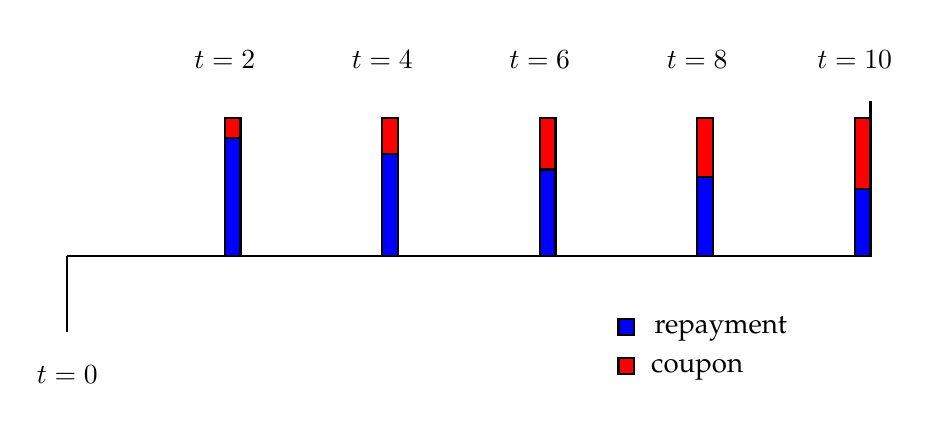
\begin{tikzpicture}[-,shorten >=1pt,auto,node distance=1.5cm,thick,minimum size=0.8cm,main node/.style={circle,draw=red,very thick}]
\tikzstyle{selected edge} = [draw,line width=6pt,-,blue!30]

\coordinate (belowstart) at (0,-1);
\coordinate (start) at (0,0);
\coordinate (stop) at (10.2,0);
\coordinate (abovestop) at (10.2,2);
\draw (start) -- (stop);
\draw (start) -- (belowstart);
\draw (stop) -- (abovestop);

\node at (0, -1.5) () {$t=0$};

\filldraw[draw=black, fill=blue] (2,0) rectangle node {} +(0.2,1.5);
\filldraw[draw=black, fill=red]  (2,1.5) rectangle node {} +(0.2,0.25);
\node at (2, 2.5) () {$t=2$};

\filldraw[draw=black, fill=blue] (4,0) rectangle node {} +(0.2,1.3);
\filldraw[draw=black, fill=red]  (4,1.3) rectangle node {} +(0.2,0.45);
\node at (4, 2.5) () {$t=4$};

\filldraw[draw=black, fill=blue] (6,0) rectangle node {} +(0.2,1.1);
\filldraw[draw=black, fill=red]  (6,1.1) rectangle node {} +(0.2,0.65);
\node at (6, 2.5) () {$t=6$};

\filldraw[draw=black, fill=blue] (8,0) rectangle node {} +(0.2,1);
\filldraw[draw=black, fill=red]  (8,1) rectangle node {} +(0.2,0.75);
\node at (8, 2.5) () {$t=8$};

\filldraw[draw=black, fill=blue] (10,0) rectangle node {} +(0.2,0.85);
\filldraw[draw=black, fill=red]  (10,0.85) rectangle node {} +(0.2,0.9);
\node at (10, 2.5) () {$t=10$};

% Legend
\filldraw[draw=black, fill=blue] (7,-1) rectangle node {} +(0.2,0.2);
\node at (8.3, -0.92) () {repayment};

\filldraw[draw=black, fill=red] (7,-1.5) rectangle node {} +(0.2,0.2);
\node at (8, -1.44) () {coupon};

\end{tikzpicture}
\caption{Cashflow of an annuity.}
\label{fig:annuitycf}
\end{center}
\end{figure}



\subsection{Bullet}

Bullet has a fixed rate coupon which is paid at every settlement. No repayments before maturity. Figure \ref{fig:bulletcf} shows the cashflows.

\[ p(t,T) = \sum_{t=1}^{T}\frac{C}{(1+r)^t} + \frac{N}{(1+r)^T} \]

\begin{figure}[h!]
\begin{center}
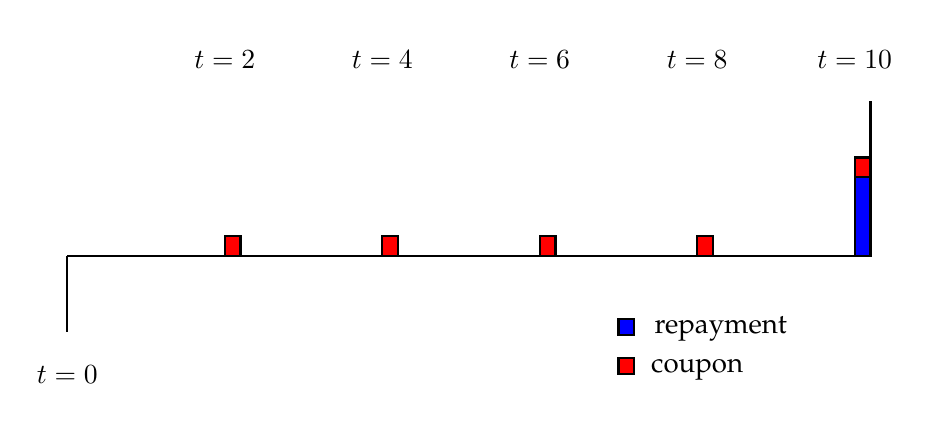
\begin{tikzpicture}[-,shorten >=1pt,auto,node distance=1.5cm,thick,minimum size=0.8cm,main node/.style={circle,draw=red,very thick}]
\tikzstyle{selected edge} = [draw,line width=6pt,-,blue!30]

\coordinate (belowstart) at (0,-1);
\coordinate (start) at (0,0);
\coordinate (stop) at (10.2,0);
\coordinate (abovestop) at (10.2,2);
\draw (start) -- (stop);
\draw (start) -- (belowstart);
\draw (stop) -- (abovestop);

\node at (0, -1.5) () {$t=0$};

\filldraw[draw=black, fill=red]  (2,0) rectangle node {} +(0.2,0.25);
\node at (2, 2.5) () {$t=2$};

\filldraw[draw=black, fill=red]  (4,0) rectangle node {} +(0.2,0.25);
\node at (4, 2.5) () {$t=4$};

\filldraw[draw=black, fill=red]  (6,0) rectangle node {} +(0.2,0.25);
\node at (6, 2.5) () {$t=6$};

\filldraw[draw=black, fill=red]  (8,0) rectangle node {} +(0.2,0.25);
\node at (8, 2.5) () {$t=8$};

\filldraw[draw=black, fill=blue] (10,0) rectangle node {} +(0.2,1);
\filldraw[draw=black, fill=red]  (10,1) rectangle node {} +(0.2,0.25);
\node at (10, 2.5) () {$t=10$};

% Legend
\filldraw[draw=black, fill=blue] (7,-1) rectangle node {} +(0.2,0.2);
\node at (8.3, -0.92) () {repayment};

\filldraw[draw=black, fill=red] (7,-1.5) rectangle node {} +(0.2,0.2);
\node at (8, -1.44) () {coupon};

\end{tikzpicture}
\caption{Cashflow of a bullet.}
\label{fig:bulletcf}
\end{center}
\end{figure}


\subsection{Consol}
Consol has a fixed rate coupon and never terminates and there is no payments at any
settlement, only interest (the coupon) is paid. Figure \ref{fig:consolcf} shows this
pictorially.

\[
p(t) = N \cdot p(t,T_n)+\sum_{i=1}^{n} (c_i \cdot p(t,T_i))
\]
\[
\lim_{x \to \infty} p(t,\infty)=\left[r\delta\sum_{i=1}^{\infty} p(t,T_i)\right]\cdot N = 
\sum_{i=0}^{\infty} p(t,T_i) \cdot \frac{\delta N}{e^{rT}} \cdot \to \frac{\delta N}{e^{rT}}\left[ \frac{e^{rT}}{r}\right] = \frac{\delta N}{r}
\]
Which means the present value of the consol bond is represented by the the following formula:
\[
p(t) = \frac{\delta N}{r}
\]

\framebox{p(t) function of time?}

\begin{figure}[h!]
\begin{center}
\begin{tikzpicture}[-,shorten >=1pt,auto,node distance=1.5cm,thick,minimum size=0.8cm,main node/.style={circle,draw=red,very thick}]
\tikzstyle{selected edge} = [draw,line width=6pt,-,blue!30]

\coordinate (belowstart) at (0,-1);
\coordinate (start) at (0,0);
\coordinate (stop) at (9.2,0);
\coordinate (dotstop) at (10.2,0);
\draw (start) -- (stop);
\draw (start) -- (belowstart);
\draw[dotted] (stop) -- (dotstop);

\node at (0, -1.5) () {$t=0$};

\filldraw[draw=black, fill=red]  (2,0) rectangle node {} +(0.2,0.25);
\node at (2, 2.5) () {$t=2$};

\filldraw[draw=black, fill=red]  (4,0) rectangle node {} +(0.2,0.25);
\node at (4, 2.5) () {$t=4$};

\filldraw[draw=black, fill=red]  (6,0) rectangle node {} +(0.2,0.25);
\node at (6, 2.5) () {$t=6$};

\filldraw[draw=black, fill=red]  (8,0) rectangle node {} +(0.2,0.25);
\node at (8, 2.5) () {$t=8$};

% Legend
\filldraw[draw=black, fill=red] (7,-1) rectangle node {} +(0.2,0.2);
\node at (8.3, -0.92) () {coupon};

\end{tikzpicture}
\caption{Cashflow of a consol.}
\label{fig:consolcf}
\end{center}
\end{figure}

\subsection{Serial}

Serial is an amortized bond with a fixed rate coupon, the repayments are spread evenly over all remaining settlements and the coupon payments, $C_t$ decline over time as depicted in figure
\ref{fig:serialcf}.

\[ p(t,T) = \sum_{t=1}^{T}\frac{C_t}{(1+r)^t} + \frac{N}{(1+r)^T} \]

\begin{figure}[h!]
\begin{center}
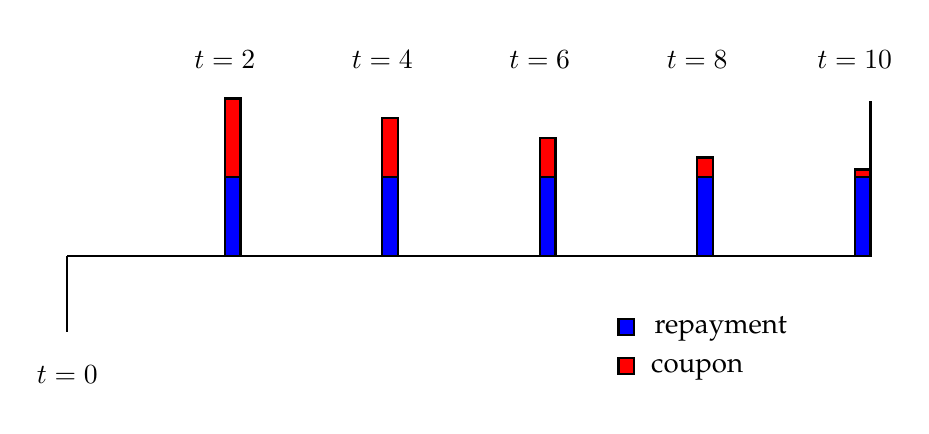
\begin{tikzpicture}[-,shorten >=1pt,auto,node distance=1.5cm,thick,minimum size=0.8cm,main node/.style={circle,draw=red,very thick}]
\tikzstyle{selected edge} = [draw,line width=6pt,-,blue!30]

\coordinate (belowstart) at (0,-1);
\coordinate (start) at (0,0);
\coordinate (stop) at (10.2,0);
\coordinate (abovestop) at (10.2,2);
\draw (start) -- (stop);
\draw (start) -- (belowstart);
\draw (stop) -- (abovestop);

\node at (0, -1.5) () {$t=0$};

\filldraw[draw=black, fill=blue] (2,0) rectangle node {} +(0.2,1);
\filldraw[draw=black, fill=red]  (2,1) rectangle node {} +(0.2,1);
\node at (2, 2.5) () {$t=2$};

\filldraw[draw=black, fill=blue] (4,0) rectangle node {} +(0.2,1);
\filldraw[draw=black, fill=red]  (4,1) rectangle node {} +(0.2,0.75);
\node at (4, 2.5) () {$t=4$};

\filldraw[draw=black, fill=blue] (6,0) rectangle node {} +(0.2,1);
\filldraw[draw=black, fill=red]  (6,1) rectangle node {} +(0.2,0.5);
\node at (6, 2.5) () {$t=6$};

\filldraw[draw=black, fill=blue] (8,0) rectangle node {} +(0.2,1);
\filldraw[draw=black, fill=red]  (8,1) rectangle node {} +(0.2,0.25);
\node at (8, 2.5) () {$t=8$};

\filldraw[draw=black, fill=blue] (10,0) rectangle node {} +(0.2,1);
\filldraw[draw=black, fill=red]  (10,1) rectangle node {} +(0.2,0.1);
\node at (10, 2.5) () {$t=10$};

% Legend
\filldraw[draw=black, fill=blue] (7,-1) rectangle node {} +(0.2,0.2);
\node at (8.3, -0.92) () {repayment};

\filldraw[draw=black, fill=red] (7,-1.5) rectangle node {} +(0.2,0.2);
\node at (8, -1.44) () {coupon};

\end{tikzpicture}
\caption{Cashflow of a serial.}
\label{fig:serialcf}
\end{center}
\end{figure}


\section{US Treasury Bonds}
Treasury securities are the debt financing instruments of the United States federal government, and they are often referred to simply as Treasuries.
\subsection{Treasury Bill - T-Bill}
Short term debt instruments that mature in one year or less.
\subsection{Treasury Note - T-Note}
Medium term debt instruments that mature in two to ten years.
\subsection{Treasury Bond - T-Bond}
Long term debt instruments that mature in twenty to thirty years.

\section{The term structure}
The term structure is defined as the zero coupon term structure.

\section{Term structure fitting methods}
Various methods of fitting a yield curve to data (LIBOR, forex futures, bonds).

\section{Interest rate swaps}
\chapter{Fixed Income Pricing}
Fixed Income Pricing (using Haskell)
\begin{itemize}
\item Haskell
\item Why Haskell etc
\item Models
\item Limitations
\end{itemize}


\chapter{Results}

\section{Evaluation}

\section{Architecture}

\section{Performance}

\section{Precision and Symbolic Computations}

\chapter{Future Work}\label{chap:fw}

Our project is far from a fully-fledged library, and many more modules must be added.

First of all we do not have support for the floating rate bonds
(see appendix X section something) due to the lack of of Monte Carlo
simulation module. A natural next step after floating rate support
would then be to implement interest rate derivatives such as swaps.

There are two obvious ways in which we can extend HQL with interest rate
derivatives support. For instance, swaps can be modelled by combining a
fixed and a floating leg, the latter still not yet being supported. On the
other hand, it could be built as a list of forward-rate agreements (make sure
this is explained above, or refer to Appendix) between the two parties in
question.\\

Alas, our library is also missing a key component which is a proper calendar
module. We currently allow the users to supply a variable number of
settlements per year. This needs to be constrained so that the users either
specify a standard settlement pattern (missing an example) or \emph{all}
payment dates for OTC products. Moreover, HQL currently assumes that all
weekdays are valid payments dates. This doesn't cater to local holidays
(e.g. January $1^{\text{st}}$ in Denmark, $4^{\text{th}}$ of July in the
United States, etc) which may be computed as offsets from Easter Sunday.\\

Another interesting extension is to implement a way of generating term
sructures from portfolios using bootstrapping and interpolation\footnote{need
a reference to Björk/Munk here}. This would essentially allow users to import
data from external sources and use HQL to build term structures and perform
bond valuation.\\

Support for mortgage-backed bonds is also missing in our library. We provide
an MBO class to be used in the future.\\
%Prepayment estimates must also be computed.

%Cubic splines or Nelson-Siegel method for obtain term structure as a function.

Finally, it would be desirable to implement an embedded domain-specific language
for construction of over-the-counter (OTC) products.
As OTC products are subject to counterparty risk, this would be another topic
to investigate.

%The class hierarchichy should be extended to define interfaces for derivatives,
%commodities, money markets etc.. Draw diagram?

\chapter{Conclusion}


%-----------------------------------------------------------
\addcontentsline{toc}{chapter}{\numberline{}Bibliography}
\bibliographystyle{plain}
\bibliography{biblio}
%-----------------------------------------------------------
\appendix
\chapter{Contributions}\ref{chap:contrib}

\newcounter{treeline}

\newcommand{\treeroot}[1]{% Title
\node[above] at (0,0) {#1};%
\setcounter{treeline}{0}
}

\newcommand{\treeentry}[2]{% Title, Level
\draw[->] (#2-1,-\value{treeline}/2) -- (#2-1,-\value{treeline}/2-0.5) -- (#2+0.5,-\value{treeline}/2-0.5) node[right] {#1};
\stepcounter{treeline}
}

\newcommand{\altentry}[2]{% Title, Level
\draw[->] (#2-1,-\value{treeline}/2) -- (#2-1,-\value{treeline}/2-0.5) -- (#2+0.5,-\value{treeline}/2-0.5) node[right] {#1};
\foreach \x in {1,...,#2}
{   \draw (\x-1,-\value{treeline}/2) -- (\x-1,-\value{treeline}/2-0.5);
}
\stepcounter{treeline}
}

\textcolor{blue}{Andreas Bock}\\
\textcolor{green}{Johan Astborg}\\
\textcolor{red}{Both}\\

\begin{tikzpicture}
\tt
\treeroot{src}
\treeentry{Instruments}{1}
\treeentry{\color{blue} Instrument.hs}{2}
\treeentry{FixedIncome}{2}
\treeentry{Bonds}{3}
\treeentry{\color{blue} Bonds.hs}{4}
\treeentry{Utils}{2}
\treeentry{\color{green} InterestRate.hs}{2}
\treeentry{\color{red} TermStructure.hs}{2}
\treeentry{Derivatives}{2}
\treeentry{\color{blue} Derivatives.hs}{3}
\treeentry{Equity}{2}
\treeentry{OTC}{2}

\treeentry{Pricing}{1}
\treeentry{Utils}{1}
\treeentry{\color{blue} Calendar.hs}{2}
\treeentry{\color{red} Currency.hs}{2}
\treeentry{\color{blue} DayCount.hs}{2}
\treeentry{Graphics}{2}
\treeentry{\color{green} Visualize.hs}{3}
\end{tikzpicture}

%-----------------------------------------------------------
\end{document}
